\documentclass{article}
\usepackage{amsmath}
\usepackage{xcolor}
\usepackage{amsthm}
\usepackage{graphicx}
\usepackage{hyperref}
\usepackage{datetime}
\usepackage{todonotes}

% inline comments
% you could use \listoftodos to print an overview
\newcommand{\inline}[1]{ {\color{blue}{#1}}\addcontentsline{tdo}{todo}{#1}}
\newcommand{\comment}[1]{{\color{blue}\noindent{#1}\\}\addcontentsline{tdo}{todo}{#1}}
% use this one to disable
%\newcommand{\inline}[1]{\ignorespaces}


\newdateformat{monthyeardate}{\monthname[\THEMONTH] \THEYEAR}

\newcommand{\newmarkedtheorem}[1]{%
  \newenvironment{#1}
    {\pushQED{\qed}\csname inner@#1\endcsname}
    {\popQED\csname endinner@#1\endcsname}%
  \newtheorem{inner@#1}%
}

\theoremstyle{definition}
%\newtheorem{eg}{Example}[section]
\newmarkedtheorem{eg}{Example}[section]
\newtheorem{observation}{Observation}[section]
\theoremstyle{plain}
\newtheorem{define}{Definition}[section]
\newtheorem{proposition}{Proposition}[section]
\newtheorem{theorem}{Theorem}[section]
\newtheorem{assump}{Assumption}[section]
\newtheorem{remark}{Remark}[section]


\title{Simple Finite Buffers}
\author{Jeroen van Riel}
\date{\monthyeardate\today}

\begin{document}

\maketitle


Assume that the ordering of vehicles is fixed for each lane, which means that
there cannot be any \textit{merging onto a lane}, where traffic from different
lanes continuous on the same lane. Stated more formally, we only allow common
paths of length one. Under this assumption, finite buffers can be easily
formulated using the followin \textit{delayed precedence constraints}.

To illustrate the idea, consider two intersections in tandem and suppose that
all vehicles follow the same route. Therefore, we can simply identify each
vehicles as $j = 1, \dots, n$ with corresponding route $R_{j} = (1, 2)$.
%
Suppose that vehicles are able to accelerate and decelerate instantaneously,
then each vehicle spends precisely $d(1, 2)$ time driving on this lane, any
additional time is spend on waiting.
%
At the crossing time $y_{ij}$, the front of vehicle $j$ is entering the
intersection zone and we assume that at time $y_{ij} + p$, the front of the
vehicle is entering the adjacent lane. Let the maximum number of vehicles that
can be at the lane between the intersections be given by a positive integer $b$.
When there are currently $b$ vehicles in the lane, we must require that a
vehicle starts leaving the lane before the next vehicle arrives to the lane,
which can be stated as
\begin{align*}
  y_{2j} \leq y_{1,j+b} + p ,
\end{align*}
for each vehicle $1 \leq j \leq n - b$.

\begin{figure}
  \centering
  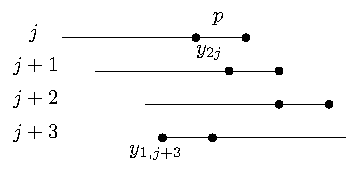
\includegraphics[width=0.6\textwidth]{figures/delayed-constraint.pdf}
  \caption{Illustration of the delayed constraint for $b=3$. Vehicle $j+3$ can
  enter the lane at $y_{1,j+3} + p$ after job $j$ enters intersection 2 at
  $y_{2j}$, ensuring there are at most $3$ vehicle on the lane at all times.}
  \label{fig:delayed-contraint}
\end{figure}

\end{document}
